\documentclass[14pt, times, a4paper]{extarticle}
\usepackage{graphicx}
\usepackage[toc,page]{appendix}
\usepackage{geometry}
\usepackage{times}
\usepackage{glossaries}
\usepackage{algorithm}
\usepackage{algorithmic}
\usepackage{tikz}
\usepackage{booktabs}
\usepackage{enumitem}
\usepackage{subcaption}
\usetikzlibrary{arrows}
\usepackage{pagecolor}
\usepackage{amsthm}
\usepackage{float}


\definecolor{covercolor}{RGB}{194,194,184}

\geometry{
    top=3.5cm,    % Adjust top margin as needed
    left=3cm, % Adjust left margin as needed
    right=2.5cm,   % Adjust right margin as needed
    bottom=2cm   % Adjust bottom margin as needed
}

\newglossaryentry{Pigeonhole Principle}{
    name={Pigeonhole Principle},
    description={If there are more pigeons than number of holes, at least one hole has more than one pigeon}
}
\newglossaryentry{traveling salesman problem}{
    name={Traveling Salesman Problem},
    description={The problem where a salseeman has to reach some places travelling minimum distance}
}
\newglossaryentry{Graph theory}{
    name={Graph theory},
    description={The study of graphs}
}
\newglossaryentry{graph}{
    name={Graph},
    description={A mathematical structure used to model pairwise relations between objects}
}

\newglossaryentry{Eulerian circuit}{
    name={Eulerian circuit},
    description={A circuit in a graph that visits every edge exactly once}
}
\newglossaryentry{Hamiltonian cycles}{
    name={Hamiltonian cycle},
    description={A cycle in a graph that visits every vertex exactly once}
}
\newglossaryentry{Euler path}{
    name={Eulerian path},
    description={A path in a graph that visits every edge exactly once}
}
\newglossaryentry{Hamiltonian path}{
    name={Hamiltonian path},
    description={A path in a graph that visits every vertex exactly once}
}
\newglossaryentry{vertex}{
    name={Vertex},
    description={A point in a graph, representing an object or concept}
}
\newglossaryentry{edge}{
    name={Edge},
    description={A connection between two vertices in a graph}
}
\newglossaryentry{cycles}{
    name={Cycle},
    description={A sequence of vertices and edges that starts and ends at the same vertex}
}
\newglossaryentry{circuit}{
    name={Circuit},
    description={A cycle in which no vertex is repeated, except for the starting and ending vertices}
}
\newglossaryentry{path}{
    name={Path},
    description={A sequence of vertices and edges that connects two vertices in a graph}
}
\newglossaryentry{Seven Bridges of Konigsberg}{
    name={Seven Bridges of Königsberg},
    description={A famous problem in graph theory that led to the development of Eulerian paths and cycles}
}
\newglossaryentry{Knight's Tour}{
    name={Knight's Tour problem},
    description={A puzzle involving finding a sequence of moves for a knight on a chessboard to visit every square exactly once}
}


\makeglossaries

\title{Euler Circuit \& Hamiltonian Cycle}
\author{Soumik Bhattacharjee \and Reduanul Islam Imon \and Tusher Bhomik}
\date{February 13, 2024}

\begin{document}


%--------------------------------------------------
%cover page
\begin{titlepage}
    %\pagecolor{covercolor}
    \centering
    \includegraphics[width=0.2\textwidth]{images/buet_logo.png}\\[1cm]
    {\Large Bangladesh University of Engineering \& Technology - BUET\par}
    \vspace{2.5cm}
    {\huge\bfseries A Simple Report on Euler Circuit \& Hamiltonian Cycle\par}
    \vspace{3cm}
    \Large
    2005031 - Soumik Bhattacharjee\\
    2005040 - Reduanul Islam Imon\\
    2005046 - Tusher Bhomik\\[2cm]
    \large
    Course Name: CSE300: Technical Writing and Presentation\\
    Group ID: 01 \hspace{2cm} Section:A2 \hspace{2cm} Dept.: CSE\\
    Date of Submission: 9th March, 2024
\end{titlepage}


%--------------------------------------------------
%frontispiece page
\pagecolor{white}
%\newpage
%\includegraphics[width=0.9\textwidth, height=0.8\textheight]{images/frontispiece_demo.jpg}
%\thispagestyle{empty}


%--------------------------------------------------
%title page
%\newpage
%\begin{titlepage}
%    \centering
%    \includegraphics[width=0.3\textwidth]{images/buet_logo.png}\\[1cm]
%    {\Large Bangladesh University of Engineering \& Technology - BUET\par}
%    \vspace{3cm}
%    {\huge\bfseries A Simple Report on Euler Circuit \& Hamiltonian Cycle\par}
%    \vspace{3cm}
%    \Large
%    2005031 - Soumik Bhattacharjee\\
%    2005040 - Reddwanul Imon\\
%    2005046 - Tusher Bhomik\\
%    Course ID: CSE300\\
%    Course Name: Technical Writing and Presentation\\
%    Date of Submission: 9th March, 2024
%\end{titlepage}


%--------------------------------------------------
%forwarding letter
\newpage
\begin{center}
    \huge Forwarding Letter
\end{center}
\vspace{1cm}

\noindent Sir,
\vspace{0.5cm}

\noindent This application is written to formally submit this report on the topic "Euler Circuit \& Hamiltonian Cycle" that we prepared for the assignment of course CSE300. As we are instructed, this report contains some basic understanding of Euler circuits and Hamiltonian cycles so that even a child can understand these concepts, along with information about some advanced features.
\vspace{0.5cm}

\noindent In case you require further information on these topics or if you have any complaints, we would request you to inform us so that we could avoid such mistakes in the near future.
\vspace{0.5cm}

\noindent Regards,
\vspace{0.5cm}

\noindent The Students of Group 1 \\
Subsection A2 \\
Batch 20\\
Department of Computer Science and Engineering


%--------------------------------------------------
%table of contents
\newpage
\tableofcontents


%------------------------------------------------
%list of illustrations
\newpage
\listoffigures


%--------------------------------------------------
%summary
\newpage
\section*{Summary}
Euler Circuit \& Hamiltonian cycle are two of the greatest contributions in graph theory and modern geometry. There are multitudinous applications based on these concepts in the present world.\\[0.3cm]
It is very easy for one to get confused on what an Euler circuit and a Hamiltonian cycle may refer to, since there are many closely related term such as an euler cycle, euler path, euler tour, euler circuit etc, Same goes for Hamiltonian cycle, circuit, path, tour. Yet, it is very easy to distinguish them from one another with using proper definition and characteristics.  An Euler circuit covers every edge in a graph exactly once and cannot use a vertex more than once, except for starting and ending vertices which are the same. On the contrary, a Hamiltonian cycle uses every vertex of a graph exactly once. Since we cannot cover same vertex twice, same edge also cannot be traversed twice.\\[0.3cm]
In this report entitled as "Euler Circuit and Hamiltonian Cycle" we have discussed fundamental graph theory concepts related to Euler circuits and Hamiltonian cycles. It provides a brief overview on this topic as well as their prerequisites for better understanding. The report discusses the properties, method of identification, history, characteristics and applications of these graphs in various fields such as computer science, mathematics, and engineering. Additionally, it delves into the connections between Euler circuits and Hamiltonian cycles, highlighting their significance in graph theory and algorithm design, as well as the ways to distinguish between the two. Through clear explanations and illustrative examples, the report aims to enhance understanding and appreciation of these important concepts.\\[0.3cm]
This report explores the concepts of Euler circuits and Hamiltonian cycles. It provides a basic understanding of these concepts, making them accessible even to those with limited prior knowledge. Additionally, the report delves into advanced features and applications of Euler circuits and Hamiltonian cycles. The report was prepared as part of the assignment for course CSE300, and it aims to provide a comprehensive overview of the topic while addressing any frequently asked questions or concerns that may arise.

%--------------------------------------------------
%introduction
\newpage
\section{Introduction}
The \gls{Graph theory}, a foundational branch of mathematics, offers invaluable insights into the structure and behavior of a variety of fields mostly in design and optimisation. At its core lie fundamental concepts such as Eulerian circuits and Hamiltonian \gls{cycles}, which are some of the key pieces in understanding the patterns and possibilities within graphs.\\[0.3cm]
Euler cycle and Euler circuit are closely related terms and often considered as the same. However, definitions from different author may vary. This is why this concept is quite vague. Some consider them as the same, while some say that an Euler circuit is not allowed to travel same vertex twice. Some may say that it is Euler cycle that cannot use a vertex twice. To remove this ambiguity, we will allow the definition of Euler cycle to use same vertex twice and will not allow that attribute for an Euler circuit.
An \gls{Eulerian circuit} traverses every \gls{edge} of a \gls{graph} exactly once, returning to the starting point while avoiding using a vertex again. This concept, pioneered by the renowned mathematician Leonhard Euler in the 18th century, illuminates the connectivity and traversability of networks, revealing hidden symmetries and pathways.\\[0.3cm]
In contrast, \gls{Hamiltonian cycles} present a different challenge, aiming to visit each \gls{vertex} of a graph exactly once, forming a closed loop. Named after Sir William Rowan Hamilton, these cycles capture the essence of exploration and traversal, offering profound implications for optimization, routing, and decision-making in various domains.\\[0.3cm]
Understanding Eulerian circuits and Hamiltonian cycles not only unveils the beauty of graph theory but also unlocks practical solutions to complex real-world problems. From designing efficient transportation networks to optimizing computer algorithms, the principles underlying these graphs permeate diverse fields, shaping our understanding of connectivity, efficiency, and complexity.\\[0.3cm]
In this report, we delve into the definitions, properties, algorithms, and applications of Eulerian circuits and Hamiltonian cycles, shedding light on their significance in contemporary mathematics, engineering, and beyond. Through exploration and analysis, we unravel the intricate threads that weave these graphs into the fabric of modern science and technology.



%--------------------------------------------------
%description
\newpage
\section{Euler Circuit}


%--------------------------------------------------
%euler intro
\subsection{Introduction to Euler Circuit}
As stated before, an \gls{Euler path} is a path on a graph which uses all edges of the graph only once. An Euler cycle is a kind of euler path that starts and ends at the same vertex. Furthermore, An Euler circuit is a kind of Euler cylce which is not allowed to use same vertex more than once. However, it can ignore vertices which has no edge connected to it. Finally, the graph which may contain an Euler cycle is called an Euler graph. This is why only limited graphs may contain an Euler circuit since the number of edges each vertex may have is either two (one incoming and one outgoing edge) or zero (not connected to an edge, so no need to reach that vertex).


%--------------------------------------------------
%euler history
\subsection{A Brief History of Euler Circuit}
The concept "Euler Circuit" originated from the famous "Seven Bridges of Konigsberg" problem. The medieval German city of Konigsberg situated on the Pregel river. The city consisted of two river banks separated by the river and two islands. The islands and banks were connected to each other by a total of seven bridges. Carl Gottlieb Ehler, a mathematician who became a mayor of a nearby city later wanted to cross every bridge exactly once. Which means he wanted to go through each of the seven bridges but he did not allow himself to pass same bridge twice. But no matter how much he tried, he could never find a solution of the problem. This is the problem later known as the "\gls{Seven Bridges of Konigsberg}" problem.
Failing to get a solution, Carl sent a letter to his friend Leonhard Euler, the famous Swiss mathematician. At first, Euler mistook it as a child's riddle and has nothing to do with math. However, he later realized that it was a problem of a section of geometry that did not even exist at that time known as geometry of lines, also known as graph theory. He invented the new section of mathematics. Considering the land sections as vertices and the bridges as edges of a graph, officially proved that the seven bridges of Konigsberg problem cannot be solved since in order to visit every edge exactly once, at most two of the vertices can be of odd degree (odd number of edges coming from a vertex). But there were four vertices all of which were of odd degree. This is why such a path was not possible to create. This is why such path was later know as a Euler path. Furthermore if the path created a circuit, it could be considered an Euler circuit. \cite{teded}\\[0.3cm]
In the letter section we will descriptively look the ins and outs for determining whether a graph contains a Euler circuit or not ?

\subsection{Properties of Euler Circuit}

\begin{itemize}
    \item \textbf{Connectivity:}\\
A fundamental property for the existence of an Euler circuit is the connectivity of the graph. In simpler terms, every vertex must be reachable from every other vertex in the graph. This requirement ensures that the circuit can traverse the entire graph without encountering isolated components. If a graph is not connected, meaning there are disjoint subgraphs, an Euler circuit cannot exist.
\begin{figure}[h]
    \begin{subfigure}{0.5\textwidth}
        \centering
        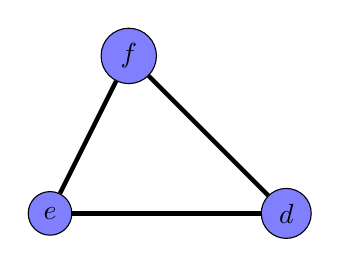
\begin{tikzpicture}
            \tikzset{vertex/.style = {shape=circle, draw, fill=blue!50, minimum size=1.5em}}
            \tikzset{edge/.style = {draw=green, ultra thick, -}}
            % vertices
            \node[vertex] (a) at  (0,0) {$e$};
            \node[vertex] (b) at  (1,2) {$f$};
            \node[vertex] (f) at  (3,0){$d$};
            % edges
            \draw[black,ultra thick] (a) to (b);
            \draw[black,ultra thick] (a) to (f);
            \draw[black,ultra thick] (b) to (f);
        \end{tikzpicture}
        \caption{Connected }
    \end{subfigure}%
    \begin{subfigure}{0.5\textwidth}
        \centering
        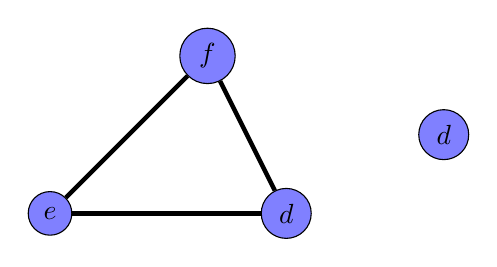
\begin{tikzpicture}
            \tikzset{vertex/.style = {shape=circle, draw, fill=blue!50, minimum size=1.5em}}
            \tikzset{edge/.style = {draw=green, ultra thick, -}}
            % vertices
            \node[vertex] (a) at  (0,0) {$e$};
            \node[vertex] (b) at  (2,2) {$f$};
            \node[vertex] (f) at  (3,0){$d$};
            \node[vertex] (g) at  (5,1){$d$};
            % edges
            \draw[black,ultra thick] (a) to (b);
            \draw[black,ultra thick] (a) to (f);
            \draw[black,ultra thick] (b) to (f);
        \end{tikzpicture}
        \caption{Not connected}
    \end{subfigure}
    \caption{Connectivity of a graph}
\end{figure}
\item \textbf{Vertex Degrees:}
All vertices in the graph must have an even degree for an Euler circuit to exist. The degree of a vertex is the number of edges incident to it. This condition is crucial because, during the traversal of the circuit, each time the circuit enters and leaves a vertex, it consumes two edges, requiring an even degree for the vertices to balance out. This property ensures that the circuit can pass through every edge without leaving any vertex unvisited.
\begin{figure}[h]
    \begin{subfigure}{0.5\textwidth}
        \centering
        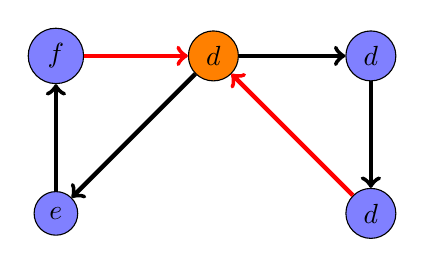
\begin{tikzpicture}
            \tikzset{vertex/.style = {shape=circle, draw, fill=blue!50, minimum size=1.5em}}
            \tikzset{edge/.style = {draw=green, ultra thick, -}}
            % vertices
            \node[vertex] (a) at  (0,0) {$e$};
            \node[vertex] (b) at  (0,2) {$f$};
            \node[vertex,fill=orange!100] (f) at  (2,2){$d$};
            \node[vertex] (g) at  (4,2){$d$};
            \node[vertex] (h) at  (4,0){$d$};
            % edges
            \draw[->,black,ultra thick] (a) to (b);
            \draw[->,black,ultra thick] (f) to (a);
            \draw[->,red,ultra thick] (b) to (f);
            \draw[->,black,ultra thick] (f) to (g);
            \draw[->,black,ultra thick] (g) to (h);
            \draw[->,red,ultra thick] (h) to (f);
        \end{tikzpicture}
        \caption{In degrees of vertex d }
    \end{subfigure}%
    \begin{subfigure}{0.5\textwidth}
        \centering
        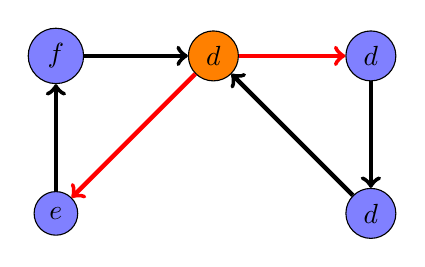
\begin{tikzpicture}
            \tikzset{vertex/.style = {shape=circle, draw, fill=blue!50, minimum size=1.5em}}
            \tikzset{edge/.style = {draw=green, ultra thick, -}}
            % vertices
            \node[vertex] (a) at  (0,0) {$e$};
            \node[vertex] (b) at  (0,2) {$f$};
            \node[vertex,fill=orange!100] (f) at  (2,2){$d$};
            \node[vertex] (g) at  (4,2){$d$};
            \node[vertex] (h) at  (4,0){$d$};
            % edges
            \draw[->,black,ultra thick] (a) to (b);
            \draw[->,red,ultra thick] (f) to (a);
            \draw[->,black,ultra thick] (b) to (f);
            \draw[->,red,ultra thick] (f) to (g);
            \draw[->,black,ultra thick] (g) to (h);
            \draw[->,black,ultra thick] (h) to (f);
        \end{tikzpicture}
        \caption{Out degrees of vertex d}
    \end{subfigure}
    \caption{Degrees Of a Vertex}
\end{figure}

\end{itemize}
\newpage

\subsection{Fleury’s Algorithm for Finding Euler Circuit}\cite{baeldung}
Fleury’s algorithm, named after Paul-Victor Fleury, a French engineer and mathematician, is a powerful tool for identifying Eulerian circuits and paths within graphs.Fleury’s algorithm is a precise and reliable method for determining whether a given graph contains Eulerian paths, circuits, or none at all. By following a series of steps, this algorithm methodically explores the graph, keeping track of the visited edges and, in the process, unveils the Eulerian structures hidden within.
\\
\\
\textbf{Theorem:}
Let $G$ be a connected graph. Fleury's Algorithm constructs an Eulerian circuit in $G$ if and only if $G$ has at most two vertices of odd degree (an odd degree means that the vertex has an odd number of edges incident to it).
\\
\\
{\bf Necessity:} If Fleury's Algorithm constructs an Eulerian circuit in $G$, then $G$ must have at most two vertices of odd degree. This is because, in an Eulerian circuit, every vertex must have an even degree to ensure that every edge is visited exactly once. The start and end vertices of the circuit may have an odd degree.
\\
\\
{\bf Sufficiency:} If $G$ has at most two vertices of odd degree, Fleury's Algorithm will construct an Eulerian circuit. The algorithm avoids bridges (edges whose removal would increase the number of connected components), ensuring that it doesn't get stuck and can traverse all edges.\\\\
\textbf{Explanation:}

This theorem essentially establishes the conditions under which Fleury's Algorithm can successfully find an Eulerian circuit. If the graph meets the degree conditions (zero or two vertices of odd degree), the algorithm is guaranteed to succeed in constructing an Eulerian circuit.

Remember that if a graph has zero vertices of odd degree, Fleury's Algorithm will construct an Eulerian circuit that starts and ends at any vertex. If it has exactly two vertices of odd degree, the algorithm will construct an Eulerian circuit that starts and ends at those two vertices.

\begin{algorithm}[H]
\caption{Fleury's Algorithm}
\label{alg:fleury}
\begin{algorithmic}[1]
\REQUIRE An Eulerian graph $G$
\ENSURE A Eulerian circuit or Eulerian path in $G$

\STATE Initialize an empty list \texttt{circuit}.
\STATE Choose a starting vertex $v$ in $G$.

\WHILE{There are unexplored edges in $G$ incident to $v$}
\STATE Let $u$ be the next vertex adjacent to $v$.
  \IF{$G$ has no other edges adjacent to $v$}
    \STATE Add $v$ to the beginning of \texttt{circuit}.
    \STATE Remove the edge between $v$ and $u$ from $G$.
  \ELSE
    \STATE Insert $v$ between $v$ and $u$ in \texttt{circuit}.
    \STATE Remove the edge between $v$ and $u$ from $G$.
  \ENDIF
\ENDWHILE
\RETURN $\texttt{circuit}$
\end{algorithmic}
\end{algorithm}
\section*{Time Complexity:}

\textbf{Worst-case:} \( \Theta((V+E)^2) \)\\
This occurs because the algorithm involves repeatedly running a depth-first search-like procedure to check for bridges within the graph. In the worst-case scenario, this edge-check might be performed for every edge, leading to a total of \( (V+E) \) iterations for a graph with \( V \) vertices and \( E \) edges. Within each iteration, another traversal might be needed to verify that a chosen edge isn't a bridge, potentially contributing another \( (V+E) \) operations. This results in a total of \( (V+E) \cdot (V+E) = \Theta((V+E)^2) \) time complexity for the worst-case scenario.\cite{geeksforgeeks}

\textbf{Average-case:} \( \Theta((V+E)^2) \)\\
The average-case time complexity is aligned with the worst-case complexity, as the algorithm involves frequent bridge-checking, potentially leading to \( (V+E)^2 \) operations even in typical cases.

\textbf{Best-case:} \( \Theta((V+E)^2) \)\\
Even in the best-case scenario, the algorithm still involves checking for bridges, resulting in a time complexity of \( \Theta((V+E)^2) \).

\section*{Space Complexity:}

\( \Theta(V^2) \)\\
The primary space consumption arises from potentially storing a list of bridges to avoid during traversal. A naive approach involves using a matrix to represent these bridges, leading to a space complexity of \( \Theta(V^2) \) for a graph with \( V \) vertices.
\subsection{An Examples and illustration of finding Euler Circuit}
\begin{itemize}
  \item Let G be Eulerian, and let C be an Euler tour of G with origin and and terminus $u$. Each time a vertex $v$ occurs as an internal vertex of C, two of the edges incident with v are accounted for. Since an Euler tour contains every edge of G, d($v$) is even for all $v \neq u$ Similarly, since C starts and ends at u, d($u$) is also even. Thus G has no vertices of odd degree.

    \begin{center}
    \begin{figure}[H]
        \centering
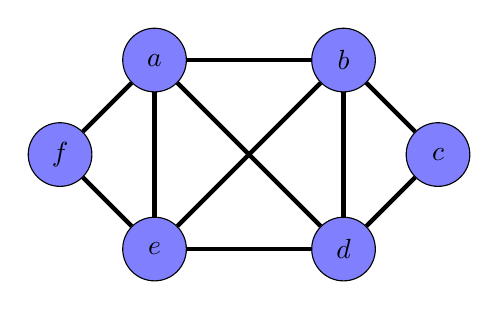
\begin{tikzpicture}[scale=0.3]
    \tikzset{vertex/.style = {shape=circle, draw, fill=blue!50, minimum size=2.3em}}
    \tikzset{edge/.style = {draw=green, ultra thick, -}}
    % vertices
    \node[vertex] (a) at  (0,0) {$e$};
    \node[vertex] (b) at  (-4,4) {$f$};
    \node[vertex] (c) at  (0,8) {$a$};
    \node[vertex] (d) at  (8,8) {$b$};
    \node[vertex] (e) at  (12,4){$c$};
    \node[vertex] (f) at  (8,0){$d$};
    % edges
    \draw[black,ultra thick] (a) to (b);
    \draw[black,ultra thick] (a) to (c);
    \draw[black,ultra thick] (a) to (d);
    \draw[black,ultra thick] (a) to (f);
    \draw[black,ultra thick] (b) to (c);
    \draw[black,ultra thick] (c) to (d);
    \draw[black,ultra thick] (c) to (f);
    \draw[black,ultra thick] (d) to (e);
    \draw[black,ultra thick] (d) to (f);
    \draw[black,ultra thick] (e) to (f);
\end{tikzpicture}
        \caption{Example of graph to find Euler curcuit}
        \label{fig:example-euler-find}
    \end{figure}
\end{center}
    
\end{itemize}
\begin{enumerate}[label=(\roman*)]

    \item Start at an arbitrary vertex $u$. Trace out a route C that never repeats an edge. Since there are no vertices of an odd degree, each vertex that is arrived at can also be left by a different edge. We created an arbitrary route C from node b in the next figure \ref{fig:failed-euler-cycle} that goes through $b \!\rightarrow\! e \!\rightarrow\! a \!\rightarrow\! d \!\rightarrow\! e \!\rightarrow\! f \!\rightarrow\! a\!\rightarrow\! b$

    \begin{center}
    \begin{figure}[H]
        \centering
    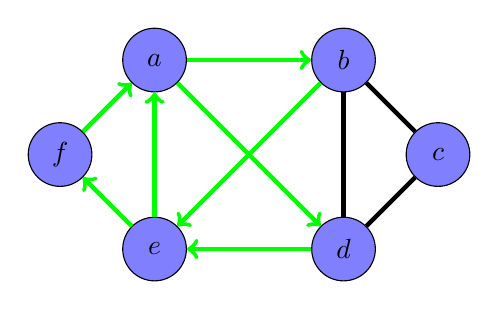
\begin{tikzpicture}[scale=0.3]
    \tikzset{vertex/.style = {shape=circle, draw, fill=blue!50, minimum size=2.3em}}
    \tikzset{edge/.style = {draw=green, ultra thick, -}}

    % vertices
    \node[vertex] (a) at  (0,0) {$e$};
    \node[vertex] (b) at  (-4,4) {$f$};
    \node[vertex] (c) at  (0,8) {$a$};
    \node[vertex] (d) at  (8,8) {$b$};
    \node[vertex] (e) at  (12,4){$c$};
    \node[vertex] (f) at  (8,0){$d$};
    
    % edges
    \draw[->,green!100,ultra thick] (a) to (b);
    \draw[->,green!100,ultra thick] (a) to (c);
    \draw[->,green!100,ultra thick] (d) to (a);
    \draw[->,green!100,ultra thick] (f) to (a);
    \draw[->,green!100,ultra thick] (b) to (c);
    \draw[->,green!100,ultra thick] (c) to (d);
    \draw[->,green!100,ultra thick] (c) to (f);
    \draw[black,ultra thick] (d) to (e);
    \draw[black,ultra thick] (d) to (f);
    \draw[black,ultra thick] (e) to (f);
    \end{tikzpicture}
    \caption{Incomplete Euler Circuit}
        \label{fig:failed-euler-cycle}
    \end{figure}
    \end{center}
    


    \item If the route does not contain all edges, choose a vertex $u'$  on C that is incident to an unused edge. Repeat step $i)$ starting at u’ and using the graph consisting only of the unused edges. Incorporate the resulting circuit into the original route C. As we can see in figure 4, the edges $bd, bc,$ and $cd$ are outside of our path C. Vertex A is incident to two of these edges. We can trace out a new route D that consists of\\ $b \!\rightarrow\! e \!\rightarrow\! a \!\rightarrow\! d \!\rightarrow\! e \!\rightarrow\! f \!\rightarrow\! a\!\rightarrow\! b\!\rightarrow\! d\!\rightarrow\! c\!\rightarrow\! b$. We can then combine path C and D, since we know there are no overlapping edges, to have a complete Euler Path that starts and ends at vertex A, as seen in figure \ref{fig:complete-euler_cycle}. 

    
    
    \begin{center}
    \begin{figure}[H]
        \centering
    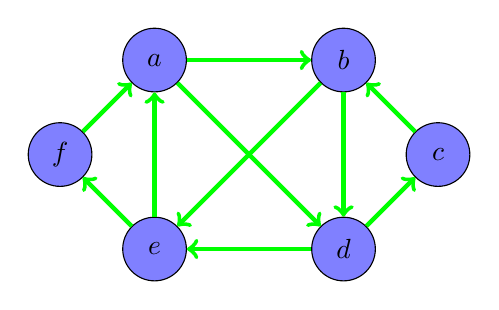
\begin{tikzpicture}[scale=0.3]
    \tikzset{vertex/.style = {shape=circle, draw, fill=blue!50, minimum size=2.3em}}
    \tikzset{edge/.style = {draw=green, ultra thick, -}}

    % vertices
    \node[vertex] (a) at  (0,0) {$e$};
    \node[vertex] (b) at  (-4,4) {$f$};
    \node[vertex] (c) at  (0,8) {$a$};
    \node[vertex] (d) at  (8,8) {$b$};
    \node[vertex] (e) at  (12,4){$c$};
    \node[vertex] (f) at  (8,0){$d$};
    
    % edges
     \draw[->,green!100,ultra thick] (a) to (b);
    \draw[->,green!100,ultra thick] (a) to (c);
    \draw[->,green!100,ultra thick] (d) to (a);
    \draw[->,green!100,ultra thick] (f) to (a);
    \draw[->,green!100,ultra thick] (b) to (c);
    \draw[->,green!100,ultra thick] (c) to (d);
    \draw[->,green!100,ultra thick] (c) to (f);
    \draw[->,green!100,ultra thick] (e) to (d);
    \draw[->,green!100,ultra thick] (d) to (f);
    \draw[->,green!100,ultra thick] (f) to (e);
    \end{tikzpicture}
    \caption{Example of an Euler Circuit}
        \label{fig:complete-euler_cycle}
    \end{figure}
    \end{center}

    \item Repeat step $(ii)$ until all edges are included in route C. Our path is complete.

\end{enumerate}
Finally, we have successfully found an Euler cycle. However, for an Euler circuit, we cannot use same vertex twice. So, there has to be only one entry point and one exit point in each vertex. This is why only the graphs with circular form, which means each vertex with degree equals to two can have an Euler circuit; just like the following graph, which is a pentagon.\cite{cite_seerx}


\subsection{Applications of Euler Circuits}

\begin{itemize}
\item Mail delivery routes: Plan an efficient route visiting every mailbox exactly once.
\item Garbage collection routes: Design a route to collect waste from every house exactly once.
\item Computer network inspection routes: Visit every switch or router exactly once for maintenance.
\item Manufacturing assembly lines: Define the order to visit stations for product assembly exactly once.
\item Solving maze puzzles: Find a path that traverses every maze passage exactly once.
\item DNA fragmentation analysis: Analyze DNA fragmentation patterns using Eulerian cycles.
\end{itemize}
%--------------------------------------------------
%description
\newpage
\section{Hamiltonian Cycle}


%--------------------------------------------------
%hamiltonian intro
\subsection{Introduction to Hamiltonian Cycle}
As stated before, a \gls{Hamiltonian path} is a path in a graph that uses every vertex exactly once. A Hamiltonian cycle is a cycle in a graph that uses every vertex exactly once. Since a Hamiltonian Path in not allowed to use same vertex twice, a Hamiltonian cycle is not a kind of Hamiltonian Path.


%--------------------------------------------------
%hamilton history
\subsection{A Brief History of Hamiltonian Cycle}
Unlike euler cycle, hamiltonian cycle is a centuries old concept. Suppose, the vertices of a graph is a landmark and the edges are the possible roads between a pair of vertices. Normally, people will definitely prioritize visiting every landmark rather than using every road. So, from a very long time, people always wanted to create such path so that one can travel every single vertex and return to the initial vertex using travelling as minimum distance as possible, which is travelling through a landmark at most once. Finding a random solution was not that difficult in simple problems. However, in complex graphs, in some cases it is not even possible to tell weather there exists such a path or not. So, researchers have always wanted to find an efficient way to find the solution.
The greatest advancement was accomplished by the hands of William Rowan Hamilton, an Irish mathematician and astronomer. His research on the famous "\gls{Knight's Tour}" problem led him to such fame and this is why the path and cycle were named after him. The Knight's Tour problem is to find the list of moves of the knight of a chessboard, starting from any arbitrary position, so that it can visit every cell of the chessboard and return to the initial position in the end. In this case, we can consider the cells as vertices and the possible destination of a knight from a vertex in a single move as edges and thus create a graph. Thus, our problem reduced to a graph problem where we have to find a Hamiltonian cycle. There are 26 trillion possible solutions to this problem and there are so many hamiltonian paths that it is still unknown to us.
Apart from this, Hamilton also devised a puzzle which requires finding a path that travels every node of a dodecahedron (consisting of 20 vertices, 30 edges and 12 pentagonal faces) once and returns to the initial position. It is the same as finding a Hamiltonian cycle in the graphical representation of the dodecahedron.  \cite{numberphile}


%--------------------------------------------------
%Imon part
\subsection{NP-Completeness:} Detecting a Hamiltonian path in a given graph is an NP complete problem i.e. we can use either backtracking or guesswork to find the solution.
\subsection{Examples and illustration}
Visual examples and illustrations of Hamiltonian cycles in different graphs can help in understanding the concept better. Here we provide some examples.

\begin{figure}[h]
  \centering
  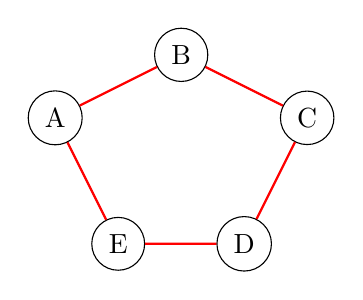
\begin{tikzpicture}[scale=0.8]
    \node[circle,draw] (A) at (0,0) {A};
    \node[circle,draw] (B) at (2,1) {B};
    \node[circle,draw] (C) at (4,0) {C};
    \node[circle,draw] (D) at (3,-2) {D};
    \node[circle,draw] (E) at (1,-2) {E};
    
    \foreach \from/\to in {A/B, B/C, C/D, D/E, E/A}
      \draw (\from) -- (\to);
      
    \draw[red,thick] (A) -- (B) -- (C) -- (D) -- (E) -- (A);
  \end{tikzpicture}
  \caption{Example of a Hamiltonian cycle in a graph with vertices A, B, C, D, and E.}
\end{figure}
\begin{figure}[h]
  \centering
  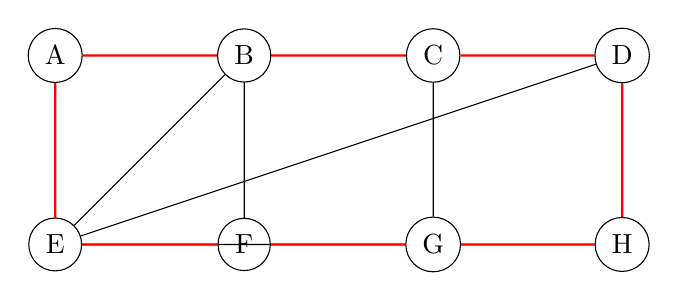
\begin{tikzpicture}[scale=1.2]
    \node[circle,draw] (A) at (0,0) {A};
    \node[circle,draw] (B) at (2,0) {B};
    \node[circle,draw] (C) at (4,0) {C};
    \node[circle,draw] (D) at (6,0) {D};
    \node[circle,draw] (E) at (0,-2) {E};
    \node[circle,draw] (F) at (2,-2) {F};
    \node[circle,draw] (G) at (4,-2) {G};
    \node[circle,draw] (H) at (6,-2) {H};
    
    \foreach \from/\to in {A/B, B/C, C/D, D/H, H/G, G/F, F/E, E/A, B/F, C/G, D/E, E/G, B/E}
      \draw (\from) -- (\to);
      
    \draw[red,thick] (A) -- (B) -- (C) -- (D) -- (H) -- (G) -- (F) -- (E) -- (A);
  \end{tikzpicture}
  \caption{Complex graph with a Hamiltonian cycle.}
\end{figure}
\subsection{Dirac's Theorem}

Dirac's theorem provides a sufficient condition for the existence of a Hamiltonian cycle in a graph:

\textbf{Dirac's Theorem}: If a graph $G$ has $n \geq 3$ vertices such that every vertex has degree at least $n/2$, then $G$ has a Hamiltonian cycle.\\

\textbf{Proof:} Suppose that G = (V, E) satisfies the hypotheses of the theorem. Then G is connected, since otherwise the degree of any vertex in a smallest component C of G would be
at most $|C| - 1 < n/2$, contradicting the hypothesis $\delta(G) \geq n/2$.
Let $P = x_0x_1$......$x_k$ be a longest path in G. Since P cannot be extended to a longer path, all the neighbours of $x_0$ and all the neighbours of $x_k$ lie on P. Hence, at least $n/2$ of
the vertices $x_0$, . . . , $x_{k-1}$ are adjacent to $x_k$, and at least $n/2$ of the vertices $x_1, . . . , x_k$ are
adjacent to $x_0$. Another way of saying the second part of the last sentence is: at least $n/2$ of the vertices $x_i \in {x_0, . . . , x_{k-1}}$ are such that $x_0x_{i+1} \in E$. Combining both statements and
using the pigeonhole principle, we see that there is some $x_i$ with $0 \leq i \leq k - 1, x_ix_k \in E$
and $x_0x_{i+1} \in E$ (see the figure \ref{fig:dirac}).
\hspace*{1cm} We claim that
\begin{equation}
    C=x_0x_{i+1}x_{i+2}......x_{k-1}x_{k}x_ix_{i-1}=x_0x_{i+1}Px_kx_iPx_0
\end{equation}
is a Hamilton cycle of G. Otherwise, since G is connected, there would be some vertex $x_j$
of C adjacent to a vertex y not in C, so that $e = x_jy \in E.$ But then we could attach e to
a path ending in $x_j$ containing k edges of C, constructing a path in G longer than P.
\begin{figure}[h]
    \centering
    \includegraphics[width=0.5\textwidth]{images/imon_graph.jpeg}
    \caption{Illustration for Dirac's Theorem}
    \label{fig:dirac}
\end{figure}
\subsection{Ore's Theorem}

Ore's theorem is another theorem that guarantees the existence of a Hamiltonian cycle in a graph:

\textbf{Ore's Theorem}: If a graph $G$ has $n \geq 3$ vertices such that for every pair of non-adjacent vertices $u$ and $v$, $\deg(u) + \deg(v) \geq n$, then $G$ has a Hamiltonian cycle.

\textbf{Proof:} From Ore's Theorem, it is not necessary to demonstrate that $G$ is connected.
Aiming for a contradiction, suppose it were possible to construct a graph that fulfills condition (1) but is not Hamiltonian.

For a given $n \geq 3$, let $G$ be the graph with the most possible edges such that $G$ is non-Hamiltonian, which satisfies condition (1).
Although it does not contain a Hamilton cycle, $G$ has to contain a Hamiltonian path $(v_1, v_2, \ldots, v_n)$.
Otherwise, it would be possible to add further edges to $G$ without making $G$ Hamiltonian.
Since $G$ is not Hamiltonian, $v_1$ is not adjacent to $v_n$, otherwise $(v_1, v_2, \ldots, v_n, v_1)$ would be a Hamilton cycle.

By condition (1), we have that:
\[ \text{deg}(v_1) + \text{deg}(v_n) \geq n \]
By the \gls{Pigeonhole Principle}, for some $i$ such that $2 \leq i \leq n-1$, $v_i$ is adjacent to $v_1$, and $v_{i-1}$ is adjacent to $v_n$.
But the cycle $(v_1, v_2, \ldots, v_{i-1}, v_n, v_{n-1}, \ldots, v_i, v_1)$ is then a Hamilton cycle.
So $G$ is Hamiltonian after all.
\subsection{Algorithms and Complexity}
\subsubsection{Approach-1: Naive Algorithm}
\begin{enumerate}
    \item Initialize a boolean matrix $\text{dp}[][]$ having dimension $N \times 2^N$, where $\text{dp}[j][i]$ represents whether there exists a path for the given subset or not.
    \item For the base case, update $\text{dp}[i][1 \ll i] = \text{true}$, for $i$ in range $[0, N - 1]$.
    \item Iterate over the range $[1, 2^N - 1]$ and perform the following steps:
    \begin{itemize}
    \item All the vertices with bits set in mask $i$ are included in the subset.
    \item Iterate over the range $[1, N]$ and let $j$ represent the end vertex of the Hamiltonian path of current subset mask $i$. Perform the following steps:
    \begin{itemize}
        \item If the value of $i$ and $2^j$ is true, then iterate over the range $[1, N]$ using variable $k$ and if the value of $\text{dp}[k][i ^{2^j}]$ is true, then mark $\text{dp}[j][i]$ as true and break out of the loop.
        \item Otherwise, continue to the next iteration.
    \end{itemize}
    \item Iterate over the range using the variable i and if the value of $\text{dp}[i][2^N - 1]$ is true, then there exists a Hamiltonian path ending at vertex $i$.
\end{itemize}
\end{enumerate}

\begin{itemize}
    \item {\textbf{Time Complexity:}The time complexity of the algorithm is $O(N \cdot 2^N)$.}
    \item {\textbf{Space Complexity:}The space complexity of the algorithm is $O(N \cdot 2^N)$.}
\end{itemize}

\clearpage
\subsubsection{Approach 2: Backtracking Algorithm}

\begin{algorithm}
\caption{Hamiltonian Cycle Backtracking Algorithm}
\begin{algorithmic}[1]
\STATE \textbf{function} \textsc{FindHamiltonianCycle}($G$)
\STATE \quad \textbf{initialize} $path$ as an empty list
\STATE \quad \textbf{return} \textsc{Backtrack}($G$, $path$, $1$)

\STATE

\STATE \textbf{function} \textsc{Backtrack}($G$, $path$, $v$)
\IF{$|path| = |V(G)|$ \textbf{and} $v$ is adjacent to the first vertex in $path$}
\RETURN $path$ concatenated with the first vertex
\ENDIF
\FOR{each vertex $u$ adjacent to $v$ in $G$}
\IF{$u$ is not in $path$}
\STATE add $u$ to $path$
\STATE $result \leftarrow$ \textsc{Backtrack}($G$, $path$, $u$) \COMMENT{Recursively explore the path}
\IF{$result$ is not \textbf{null}}
\RETURN $result$
\ENDIF
\STATE remove $u$ from $path$ \COMMENT{Backtrack}
\ENDIF
\ENDFOR
\RETURN \textbf{null}
\end{algorithmic}
\end{algorithm}
\cite{cormen2009introduction}
\begin{itemize}
    \item {\textbf{Example for Backtracking Algorithm:}

Consider the following graph:

\begin{figure}[h]
  \centering
  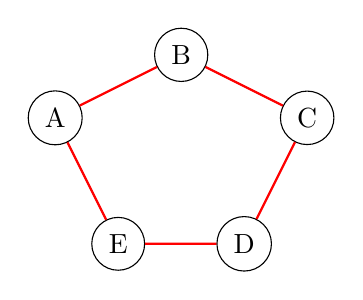
\begin{tikzpicture}[scale=0.8]
    \node[circle,draw] (A) at (0,0) {A};
    \node[circle,draw] (B) at (2,1) {B};
    \node[circle,draw] (C) at (4,0) {C};
    \node[circle,draw] (D) at (3,-2) {D};
    \node[circle,draw] (E) at (1,-2) {E};
    
    \foreach \from/\to in {A/B, B/C, C/D, D/E, E/A}
      \draw (\from) -- (\to);
      
    \draw[red,thick] (A) -- (B) -- (C) -- (D) -- (E) -- (A);
  \end{tikzpicture}
  \caption{Example of a graph with vertices A, B, C, D, and E.}
\end{figure}}
\item {\textbf{Explanation of Algorithm Steps:}We will apply the backtracking algorithm to find a Hamiltonian cycle in this graph.

\begin{enumerate}
    \item We start the algorithm by calling the \textsc{FindHamiltonianCycle} function with the given graph $G$.
    \item The \textsc{Backtrack} function is called recursively from the starting vertex $A$.
    \item We explore all possible paths from vertex $A$ to other vertices using a depth-first search approach.
    \item At each step, we add the current vertex to the path and recursively explore the paths from adjacent vertices.
    \item If a Hamiltonian cycle is found, the algorithm returns the cycle; otherwise, it backtracks and explores other paths.
    \item In this specific graph, the algorithm will find the Hamiltonian cycle $ABCDEA$.
\end{enumerate}}
\end{itemize}
\begin{itemize}
    \item {\textbf{Time Complexity:}}
The time complexity of the Hamiltonian cycle backtracking algorithm depends on the number of vertices and edges in the graph. In the worst case, the algorithm explores all possible permutations of vertices, which results in a time complexity of $O(n!)$, where $n$ is the number of vertices in the graph.
\item {\textbf{Space Complexity:}}
Since we are not using any auxiliary space, the space complexity for finding the Hamiltonian Cycle using Backtracking approach is O(1).
\end{itemize}

\subsection{Applications}

Hamiltonian cycles have various applications in different fields:

\begin{itemize}
  \item Optimization problems, such as the \gls{traveling salesman problem}, can be formulated using Hamiltonian cycles.
  \item In robotics, Hamiltonian cycles are used for path planning, ensuring that a robot visits all required locations without revisiting any.
  \item Hamiltonian cycles are also applied in network routing algorithms.
  \item In bioinformatics, Hamiltonian cycles are utilized in DNA sequencing algorithms.
\end{itemize}


%--------------------------------------------------
%conclusion
\newpage
\section{Conclusion}
In conclusion, our exploration of Euler circuits and Hamiltonian cycles has shed light on fundamental concepts in graph theory with profound implications across various disciplines. Through our investigation, we have elucidated the defining characteristics of Euler circuits, which traverse each edge of a graph exactly once, and Hamiltonian cycles, which visit each vertex exactly once. These concepts serve as the cornerstone of modern graph theory, enabling the analysis and optimization of complex networks and systems.\\[0.3cm]
Our examination of Euler circuits and Hamiltonian cycles has revealed their ubiquitous presence in real-world applications, ranging from transportation networks to computer algorithms. Understanding and harnessing the properties of these circuits and cycles offer valuable insights into the connectivity and structure of networks, facilitating efficient routing, resource allocation, and problem-solving.\\[0.3cm]
Furthermore, our report has highlighted the interplay between Euler circuits and Hamiltonian cycles, illustrating how their properties intersect and diverge in different contexts. By exploring advanced features and applications, we have demonstrated the versatility and adaptability of these concepts in addressing diverse challenges across domains.\\[0.3cm]
As we conclude our study, it becomes evident that Euler circuits and Hamiltonian cycles represent not only theoretical constructs but also powerful tools for analysis and optimization in practical settings. Their exploration opens avenues for further research and innovation, promising continued advancements in graph theory and its applications.\\[0.3cm]
In summary, our report on Euler circuits and Hamiltonian cycles underscores the importance of these concepts in understanding the structure and behavior of networks. By providing a comprehensive overview and analysis, we hope to inspire further exploration and utilization of these fundamental principles in both academic research and real-world problem-solving.


%--------------------------------------------------
%recommendation
\newpage
\section{Recommendations}
\begin{description}
    \item[Further Research:] As stated, before, Euler circuit and Hamiltonian Cycle is greatly beneficial. This is why more efficient algorithms should be developed. Besides, Hamiltonian cycle being an NP complete problem, solving it in polynomial time can bring a revolutionary change in computer science as well as our day to day life. This is why researches are being conducted to make it possible.
    
    \item[Education and Training:] Promoting education and training programs on graph theory, particularly focusing on Euler circuits and Hamiltonian cycles, can enhance the understanding and proficiency of students, researchers, and practitioners. Workshops, seminars, and online courses can provide valuable knowledge and practical skills in graph theory.
    
    \item[Algorithm Optimization:] Continuously refining and optimizing algorithms for identifying Euler circuits and Hamiltonian cycles can lead to improved efficiency and scalability in various applications, such as network routing, logistics optimization, and DNA sequencing. Collaborative research initiatives and open-source development efforts can facilitate the sharing of knowledge and resources to advance algorithmic techniques.
    
    \item[Real-world Applications:] Euler circuits and Hamiltonian cycles are unknowingly integrated to our life. Transportation, telecommunications, and computer networks use graph theory for innovation and optimization. So, these circuits and cycles should be developed in every sector as much as possible. The resources in the world are limited. So, it is necessary to ensure optimal usage of everything. This is where Euler circuit and Hamiltonian cycle can help in finding ways of using resources optimally.
    
    \item[Standardization and Best Practices:] Establishing standardized methodologies and best practices for analyzing and implementing Euler circuits and Hamiltonian cycles can promote consistency and interoperability across different domains and applications. Professional organizations and standards bodies can play a pivotal role in developing guidelines and frameworks to support industry-wide adoption and collaboration.
\end{description}



%--------------------------------------------------
%appendix
%\newpage
%\appendix % Start of appendix section
%\begin{appendices}
%\section{Appendix A}
% Content for Appendix A

%\section{Appendix B}
% Content for Appendix B
%\end{appendices}

%--------------------------------------------------
%list of references
\newpage
\setcounter{section}{6}
\addcontentsline{toc}{section}{\protect\numberline{\thesection}References}
\bibliographystyle{plain}
\bibliography{references}


%--------------------------------------------------
%glossary
\newpage
\setcounter{section}{7}
\addcontentsline{toc}{section}{\protect\numberline{\thesection}Glossary}
\printglossaries


%--------------------------------------------------
\end{document}